\documentclass[./../main.tex]{subfiles}
\graphicspath{{img/}}

\begin{document}
    \section{}

    Considerar el campo de desplazamientos definido por:

    \begin{equation*}
        \vect{u}(x, y, t) = u(x, y, t)\ex + v(x, y, t)\ey
    \end{equation*}

    donde

    \begin{alignat*}{2}
        u(x, y, t) &= \sin\bigl(\tfrac{2\pi x}{L}\bigr)\cos\bigl(\tfrac{2\pi y}{L}\bigr) &\qquad\qquad & v = -\cos\bigl(\tfrac{2\pi x}{L}\bigr)\sin\bigl(\tfrac{2\pi y}{L}\bigr) \\
    \end{alignat*}

    en el dominio \(0 \leq x \leq L_{x} = 1\), \(0 \leq y \leq L_{y} = 1\).
    
    Determinar:

    \begin{enumerate}[label=\arabic*)]
        \item el tensor de gradiente del campo de desplazamientos,
        
        Sabemos que el tensor de gradiente del campo de desplazamientos se obtiene a partir de 

        \begin{equation*}
            \grad{\vect{u}} =
            \begin{bNiceMatrix}
                \pdv{u}{x} & \pdv{u}{y} & \pdv{u}{z} \\
                \pdv{v}{x} & \pdv{v}{y} & \pdv{v}{z} \\
                \pdv{w}{x} & \pdv{w}{y} & \pdv{w}{z}
            \end{bNiceMatrix}
        \end{equation*}

        pero como nuestro campo no tiene componente en la dirección de \(\ez\), entonces

        \begin{equation*}
            \grad{\vect{u}} =
            \begin{bNiceMatrix}
                \pdv{u}{x} & \pdv{u}{y} & 0 \\
                \pdv{v}{x} & \pdv{v}{y} & 0 \\
                0 & 0 & 0
            \end{bNiceMatrix}
        \end{equation*}

        Calculando cada una de las componentes, se tiene que

        \begin{alignat*}{2}
            \pdv{u}{x} &= \tfrac{2\pi}{L}\cos\bigl(\tfrac{2\pi x}{L}\bigr)\cos\bigl(\tfrac{2\pi y}{L}\bigr)\qquad\qquad \pdv{u}{y}&{}={}& -\tfrac{2\pi}{L}\sin\bigl(\tfrac{2\pi x}{L}\bigr)\sin\bigl(\tfrac{2\pi y}{L}\bigr) \\
            \pdv{v}{x} &= \tfrac{2\pi}{L}\sin\bigl(\tfrac{2\pi x}{L}\bigr)\sin\bigl(\tfrac{2\pi y}{L}\bigr)\qquad\qquad \pdv{v}{y}&{}={}& -\tfrac{2\pi}{L}\cos\bigl(\tfrac{2\pi x}{L}\bigr)\cos\bigl(\tfrac{2\pi y}{L}\bigr).
        \end{alignat*}

        Por lo que \(\grad{\vect{u}}\) queda como

        \begin{empheq}[box=\resultbox]{equation*}
            \grad{\vect{u}} = 
            \tfrac{2\pi}{L}
            \begin{bNiceMatrix}
                \cos\bigl(\tfrac{2\pi x}{L}\bigr)\cos\bigl(\tfrac{2\pi y}{L}\bigr) & -\sin\bigl(\tfrac{2\pi x}{L}\bigr)\sin\bigl(\tfrac{2\pi y}{L}\bigr) & 0 \\
                \sin\bigl(\tfrac{2\pi x}{L}\bigr)\sin\bigl(\tfrac{2\pi y}{L}\bigr) & -\cos\bigl(\tfrac{2\pi x}{L}\bigr)\cos\bigl(\tfrac{2\pi y}{L}\bigr) & 0 \\
                0 & 0 & 0
            \end{bNiceMatrix}.
        \end{empheq}
        
        \item el tensor de deformación (parte simétrica del gradiente del campo de desplazamientos),
        
        Recordemos que el tensor gradiente del campo de desplazamientos puede escribirse como

        \begin{equation*}
            \grad{\vect{u}} = \tfrac{1}{2}\bigl(\grad{\vect{u}} + (\grad{\vect{u}})^{T}\bigr) + \tfrac{1}{2}\bigl(\grad{\vect{u}} - (\grad{\vect{u}})^{T}\bigr),
        \end{equation*}

        donde el tensor de deformación \(\varepsilon_{ij}\) es

        \begin{equation}
            \varepsilon_{ij} = \tfrac{1}{2}(u_{i,j} + u_{j,i})
            \label{eq:deformation_tensor}
        \end{equation}

        y el tensor de rotación \(\omega_{ij}\) es

        \begin{equation}
            \omega_{ij} = \tfrac{1}{2}(u_{i,j} - u_{j,i}).
            \label{eq:rotation_tensor}
        \end{equation}

        Queremos obtener \cref{eq:deformation_tensor}, pero nos podemos ahorrar algunos cálculos debido a nuestra definición del campo de desplazamientos pues las componentes para las cuales \(i = 3\) o \(j = 3\) serán cero, \emph{i.e.},

        \begin{equation*}
            \varepsilon_{13} = \varepsilon_{23} = \varepsilon_{3i} = 0.
        \end{equation*}

        Así,

        \begin{align*}
            \varepsilon_{xx} &= \pdv{u}{x} = \tfrac{2\pi}{L}\cos\bigl(\tfrac{2\pi x}{L}\bigr)\cos\bigl(\tfrac{2\pi y}{L}\bigr),\\
            \varepsilon_{xy} &= \tfrac{1}{2}\Bigl(\pdv{u}{y} + \pdv{v}{x}\Bigr) = \tfrac{1}{2}\Bigl(\sin\bigl(\tfrac{2\pi x}{L}\bigr)\sin\bigl(\tfrac{2\pi y}{L}\bigr) - \sin\bigl(\tfrac{2\pi x}{L}\bigr)\sin\bigl(\tfrac{2\pi y}{L}\bigr)\Bigr) = 0 = \varepsilon_{yx},\\
            \varepsilon_{yy} &= \pdv{v}{y} = -\tfrac{2\pi}{L}\cos\bigl(\tfrac{2\pi x}{L}\bigr)\cos\bigl(\tfrac{2\pi y}{L}\bigr).
        \end{align*}

        Así, el tensor de deformación queda como

        \begin{empheq}[box=\resultbox]{equation*}
            \dbloverline{\varepsilon} = \tfrac{2\pi}{L}
            \begin{bNiceMatrix}
                \cos\bigl(\tfrac{2\pi x}{L}\bigr)\cos\bigl(\tfrac{2\pi y}{L}\bigr) & 0 & 0 \\
                0 & -\cos\bigl(\tfrac{2\pi x}{L}\bigr)\cos\bigl(\tfrac{2\pi y}{L}\bigr) & 0 \\
                0 & 0 & 0
            \end{bNiceMatrix}.
        \end{empheq}
        
        \item el tensor de rotación (parte antisimétrica del gradiente del campo de desplazamientos),
        
        Para obtener el tensor de rotación lo hacemos a partir de \cref{eq:rotation_tensor}. Nos ``ahorramos'' nuevamente algunos cálculos pues sabemos que \(\omega_{ij}\) para \(i = j\) y que las componentes cuando \(i = 3\) o \(j = 3\) serán cero, lo cual nos deja únicamente con las componentes \(\omega_{12}\) y \(\omega_{21}\) pero \(\omega_{12} = -\omega_{21}\). Entonces,

        \begin{equation*}
            \omega_{12} = \tfrac{1}{2}\Bigl(\pdv{u}{y} -\pdv{v}{x}\Bigr) = -\tfrac{2\pi}{L}\sin\bigl(\tfrac{2\pi x}{L}\bigr)\sin\bigl(\tfrac{2\pi y}{L}\bigr) = -\omega_{21}.
        \end{equation*}

        Por lo que el tensor de rotación queda como

        \begin{empheq}[box=\resultbox]{equation*}
            \dbloverline{\omega} = \tfrac{2\pi}{L}
            \begin{bNiceMatrix}
                0 & -\sin\bigl(\tfrac{2\pi x}{L}\bigr)\sin\bigl(\tfrac{2\pi y}{L}\bigr) & 0 \\
                \sin\bigl(\tfrac{2\pi x}{L}\bigr)\sin\bigl(\tfrac{2\pi y}{L}\bigr) & 0 & 0 \\
                0 & 0 & 0
            \end{bNiceMatrix}.
        \end{empheq}
        
        \item el vector de rotación,
        
        Calculamos el vector de rotación \(\vect{\omega}_{*}\) definido como 

        \begin{equation*}
            \vect{\omega}_{*} = \curl{\vect{u}},
        \end{equation*}

        tal que,

        \begin{align*}
            \vect{\omega}_{*} &= \begin{multlined}[t]
            \begin{vNiceMatrix}[baseline=3]
                \ex & \ey & \ez \\
                \pdv{}{x} & \pdv{}{y} & \pdv{}{z}\\
                \sin\bigl(\tfrac{2\pi x}{L}\bigr)\cos\bigl(\tfrac{2\pi y}{L}\bigr) & -\cos\bigl(\tfrac{2\pi x}{L}\bigr)\sin\bigl(\tfrac{2\pi y}{L}\bigr) & 0
            \end{vNiceMatrix},\end{multlined}\\
            &= \ex\Bigl(\pdv{w}{z}\Bigr) - \ey\Bigl(-\pdv{u}{z}\Bigr) + \ez\Bigl(\pdv{v}{x} - \pdv{u}{y}\Bigr),\\
            &= \tfrac{2\pi}{L}\Bigl(\sin\bigl(\tfrac{2\pi x}{L}\bigr)\sin\bigl(\tfrac{2\pi y}{L}\bigr) + \sin\bigl(\tfrac{2\pi x}{L}\bigr)\sin\bigl(\tfrac{2\pi y}{L}\bigr)\Bigr)\ez,\\
            \Aboxedmain{
                \vect{\omega}_{*} &= \Bigl(0, 0, \tfrac{4\pi}{L}\sin\bigl(\tfrac{2\pi x}{L}\bigr)\sin\bigl(\tfrac{2\pi y}{L}\bigr)\Bigr).
            }
        \end{align*}
        
        \item la divergencia. 
        
        La divergencia la calculamos como

        \begin{align*}
            \dvg{\vect{u}} &= \pdv{u}{x} + \pdv{v}{y},\\
            &= \tfrac{2\pi}{L}\Bigl(\cos\bigl(\tfrac{2\pi x}{L}\bigr)\cos\bigl(\tfrac{2\pi y}{L}\bigr) - \cos\bigl(\tfrac{2\pi x}{L}\bigr)\cos\bigl(\tfrac{2\pi y}{L}\bigr)\Bigr),\\
            \Aboxedmain{
                \dvg{\vect{u}} &= 0.
            }
        \end{align*}
    \end{enumerate}

    \pagebreak
    Graficar:

    \begin{enumerate}[resume, label=\arabic*)]
        \item campo de desplazamientos,
        
        La gráfica del campo de desplazamientos se muestra en la \cref{fig:displacement_field}.

        \begin{figure}[htb]
            \centering
            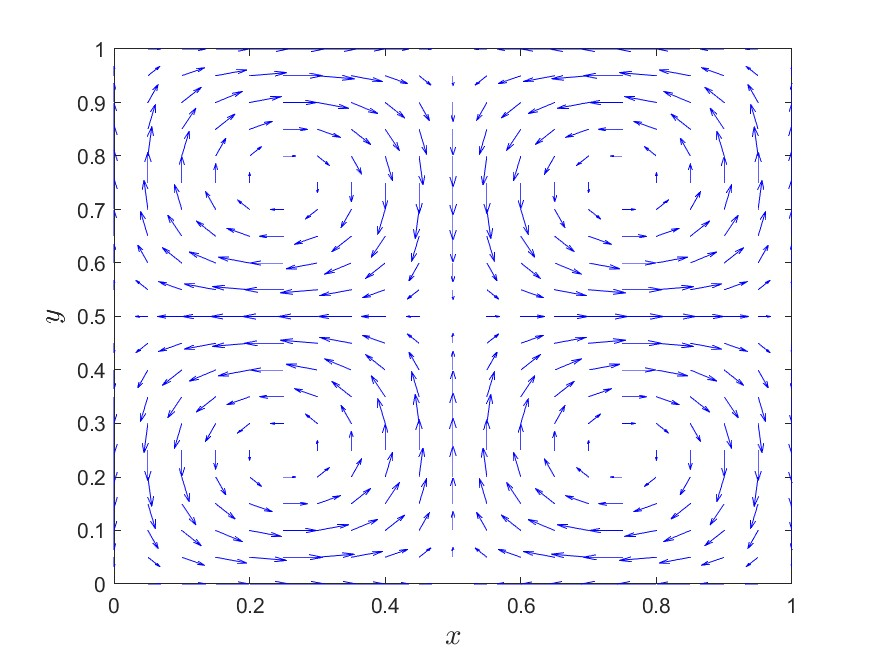
\includegraphics[width=0.55\textwidth]{campo-desplazamientos.jpg}
            \caption{Gráfica del campo de desplazamientos.}
            \label{fig:displacement_field}
        \end{figure}
        
        \item vector de rotación (nota: considerar como un campo escalar).
        
        La gráfica del vector de rotación se muestra en la \cref{fig:rotation_vector}.

        \begin{figure}[htb]
            \centering
            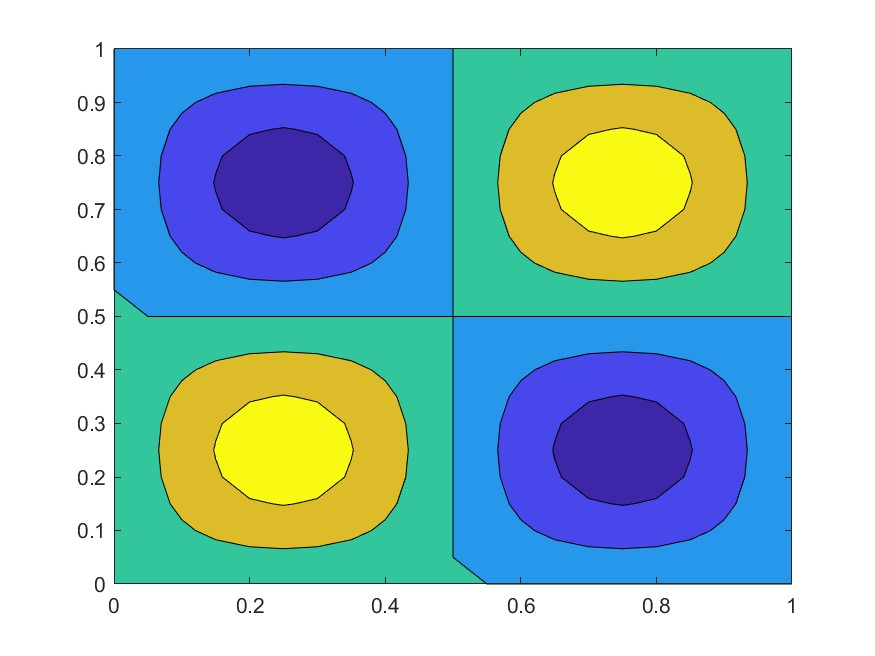
\includegraphics[width=0.55\textwidth]{vector-rotacion.jpg}
            \caption{Gráfica del vector de rotación.}
            \label{fig:rotation_vector}
        \end{figure}
    \end{enumerate}
\end{document}